\chapter{Fonctionnement en mode autonome}

\section{Présentation}

L'application Filo-Science peut fonctionner en mode autonome, c'est à dire sans connexion internet. Le principe est décrit dans la figure \ref{fig:docker}.

\begin{figure}[h]
\centering
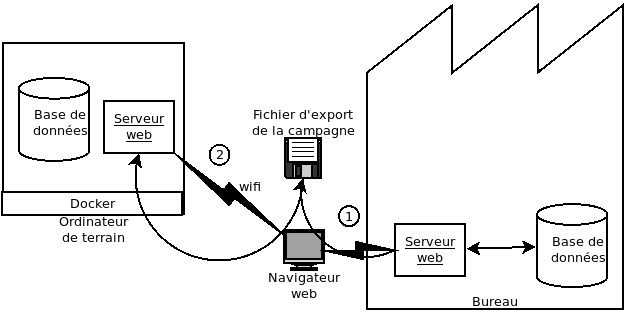
\includegraphics[width=0.8\linewidth]{images/docker_schema_general}
\caption{Schéma général de fonctionnement du mode autonome.}
\label{fig:docker}
\end{figure}

Dans un premier temps, les informations générales sur la campagne sont saisies dans l'application centrale (bureau), ainsi que les informations liées au projet. La campagne est ensuite exportée (modèle d'export : \textit{Description des campagnes}) dans un fichier au format JSON.

Dans un second temps, l'application est installée dans une machine destinée à aller sur le terrain (ordinateur portable Windows, ou couple Raspberry\footnote{Les Raspberry sont des ordinateurs de très petite taille (ils tiennent dans une poche), fonctionnant sans écran ni clavier, destinés à être utilisés un peu partout, et peu chers (quelques dizaines d'euros, moins de 150 euros avec une batterie). Ils fonctionnent avec un système d'exploitation basé sur Linux, et embarquent un émetteur wifi permettant de connecter une tablette, par exemple.} -- tablette Android). 
Un navigateur se connecte au serveur web embarqué qui contient une copie de l'application. À partir de celle-ci, il suffit d'importer le fichier généré précédemment pour récupérer les paramètres du projet et de la campagne.

La saisie s'effectue alors à partir du système autonome. Une fois la campagne terminée, il faut réaliser les opérations dans l'autre sens :  les saisies faites sur le terrain sont exportées au format JSON depuis l'application embarquée (depuis le détail de la campagne, liste des opérations réalisées), puis importées dans l'application centrale.

\section{Installer l'application et la base de données dans un matériel autonome}

L'installation a été prévue pour utiliser un composant particulier, \textit{Docker}, qui permet d'installer n'importe quel système sur n'importe quel autre, tout en gardant le paramétrage particulier du premier.

L'ensemble de la procédure d'installation, à la fois de Docker, de l'application et de la base de données est décrite (en anglais et en français) dans un projet \textit{Github} : \href{https://github.com/Irstea/filo-docker}{https://github.com/Irstea/filo-docker}.
Des instructions particulières concernent l'installation dans un Raspberry, avec l'activation du wifi pour pouvoir connecter une tablette.

